\RequirePackage[l2tabu, orthodox]{nag} % generates warnings for stuff you shouldn't do
\documentclass[conference]{IEEEtran}

\usepackage[utf8]{inputenc}
\usepackage{multirow} % Allows for multiple rows
\usepackage{multicol} % Allows for multiple columns
\PassOptionsToPackage{hyphens}{url}\usepackage[hidelinks]{hyperref}	% Breaks URLs down and allows the document to link to sections

% Bibliography preamble
\usepackage[style=apa,backend=biber,sorting=none]{biblatex}	% APA style biblatex
\addbibresource{references.bib}		% Path of the library

% Images preamble
\usepackage{graphicx}				% Import graphics
% \graphicspath{ {./img/} }	        % Set path to images
\usepackage{wrapfig}			    % Wrap figure around text
\usepackage{tikz}				    % Draw shapes
\usetikzlibrary{positioning,chains} % Libraries used by Tikz
\usepackage{float}					% Correcting the positioning of images
\usepackage{adjustbox}				% Wrapper for images
\usepackage[labelfont=bf]{caption}	% Caption generated text
\usepackage{subcaption}				% Allow sub captions


\title{Automatic Detection of Mind Wandering from Multimodal Datastreams:\\ 
A Survey of State-of-the-art Methods}
\author{Murtadha Al Nahadi, Robin Faber, Justin de Haan, Wessel Turk}
\date{March 2019}


\begin{document}
\maketitle
\begin{abstract}
    This document is a model and instructions for \LaTeX.
    This and the IEEEtran.cls file define the components of your paper [title, text, heads, etc.]. *CRITICAL: Do Not Use Symbols, Special Characters, Footnotes, 
    or Math in Paper Title or Abstract.
    \end{abstract}
    
    \begin{IEEEkeywords}
    component, formatting, style, styling, insert
    \end{IEEEkeywords}


\section{Introduction}
Lorem ipsum dolor sit amet, consectetur adipiscing elit. Suspendisse interdum arcu sit amet erat rutrum pulvinar sed eget lectus. Donec id neque diam. Orci varius natoque penatibus et magnis dis parturient montes, nascetur ridiculus mus. In nec cursus nibh, vel lacinia libero. Donec faucibus ornare finibus. Proin hendrerit sagittis magna, eget commodo mauris pulvinar id. Sed tincidunt massa eget ex ultricies bibendum sed vel elit. Ut varius posuere consequat. Curabitur rutrum metus sit amet malesuada sollicitudin. Donec ac mollis velit. Pellentesque fringilla sodales finibus. Donec pellentesque a ipsum at interdum.

Aenean tincidunt condimentum convallis. Aliquam volutpat lorem at risus varius, eu gravida est fringilla. Mauris vestibulum justo libero, sit amet dapibus lorem tempus eget. Morbi nec viverra leo. Nullam ut vestibulum mi, sed maximus quam. Integer dapibus, ex et cursus imperdiet, massa tortor volutpat eros, sed ultricies velit libero et turpis. Nullam rutrum, mauris in commodo ornare, est lorem dapibus tellus, eu aliquam arcu risus ornare est.

Maecenas non sagittis neque. Donec convallis, tellus consectetur fringilla eleifend, arcu risus tristique eros, nec iaculis metus justo vitae lorem. Nam imperdiet tellus pretium justo auctor, vitae maximus metus faucibus. Aliquam vel arcu sagittis, lobortis arcu et, placerat felis. Sed nec volutpat lorem. Mauris purus est, placerat et nisl quis, venenatis vestibulum eros. Suspendisse convallis nisi eu nisl ultrices, eu dignissim mauris sagittis. Nam odio dui, accumsan at eros dictum, convallis efficitur nunc. Sed lobortis felis felis. Mauris ullamcorper tristique nulla nec bibendum. Nulla dapibus lobortis vestibulum. Donec eget lectus sed tellus euismod ultricies nec non justo. Nullam tincidunt, lorem non pellentesque sollicitudin, enim enim accumsan orci, et dignissim purus felis et mauris. Maecenas faucibus vehicula tellus a semper. Proin eu eleifend eros, ac lobortis urna.

Aliquam vel pretium dui. Vestibulum placerat quam vel imperdiet blandit. Donec convallis, neque id molestie ornare, nulla mi convallis sapien, in fermentum purus erat eu velit. Donec efficitur rhoncus tellus, eu semper eros consequat sit amet. Donec aliquam lacinia velit nec mollis. Sed quis mi vel urna blandit vehicula sed ac velit. Nam metus eros, congue laoreet condimentum eu, porttitor a enim. Proin placerat ornare metus, scelerisque placerat est gravida quis. Aliquam vitae arcu ullamcorper risus viverra suscipit at et elit. Pellentesque rhoncus ultrices enim sed semper.

Quisque facilisis, dolor gravida iaculis tincidunt, turpis ante sodales lectus, et semper nibh nunc vitae augue. Vivamus at dui vel purus fringilla ultrices id ut dolor. Nulla a pulvinar orci. Praesent efficitur molestie orci, eget dictum risus lobortis ac. Vestibulum varius turpis ut ipsum ullamcorper ullamcorper. Vivamus lacinia mi quis nulla malesuada, vel laoreet tellus scelerisque. Cras sapien ipsum, feugiat ac neque vitae, mollis molestie tortor. Aliquam a fringilla arcu. Suspendisse in nisi consequat, congue arcu quis, dapibus sapien. Praesent quis dui nibh. Nam iaculis et purus quis porttitor. Sed aliquet erat quis iaculis consequat. Nulla ligula ipsum, congue in scelerisque a, volutpat ac urna.

\section{Definition of Mind Wandering}

\section{Detection of Mind Wandering}

\section{Methodology}


In order to gather all relevant articles needed to perform this state-of-the-art review, a systematic approach was used (figure \ref{fig:prisma}).

First, 10 articles were hand-picked that were identified as relevant to the subject. These hand-picked articles served as a baseline for the upcoming search in online libraries.
A systematic search on Scopus and Web of Science was performed to identify all articles aimed at the detection of mind wandering. The retrieved articles were checked on relevancy and completeness.
An indication on the completeness of the search terms was obtained by comparing the results of the online libraries with the baseline. 
The used search terms were tweaked by making them broader when the results did not contain a lot of the baseline articles, and made narrower when there were many irrelavant articles retrieved.
*A logbook of the used search terms can be found in appendix A.*
As a result of this first step an initial list of 129 articles was obtained.

\begin{figure}
  \resizebox{\columnwidth}{!}{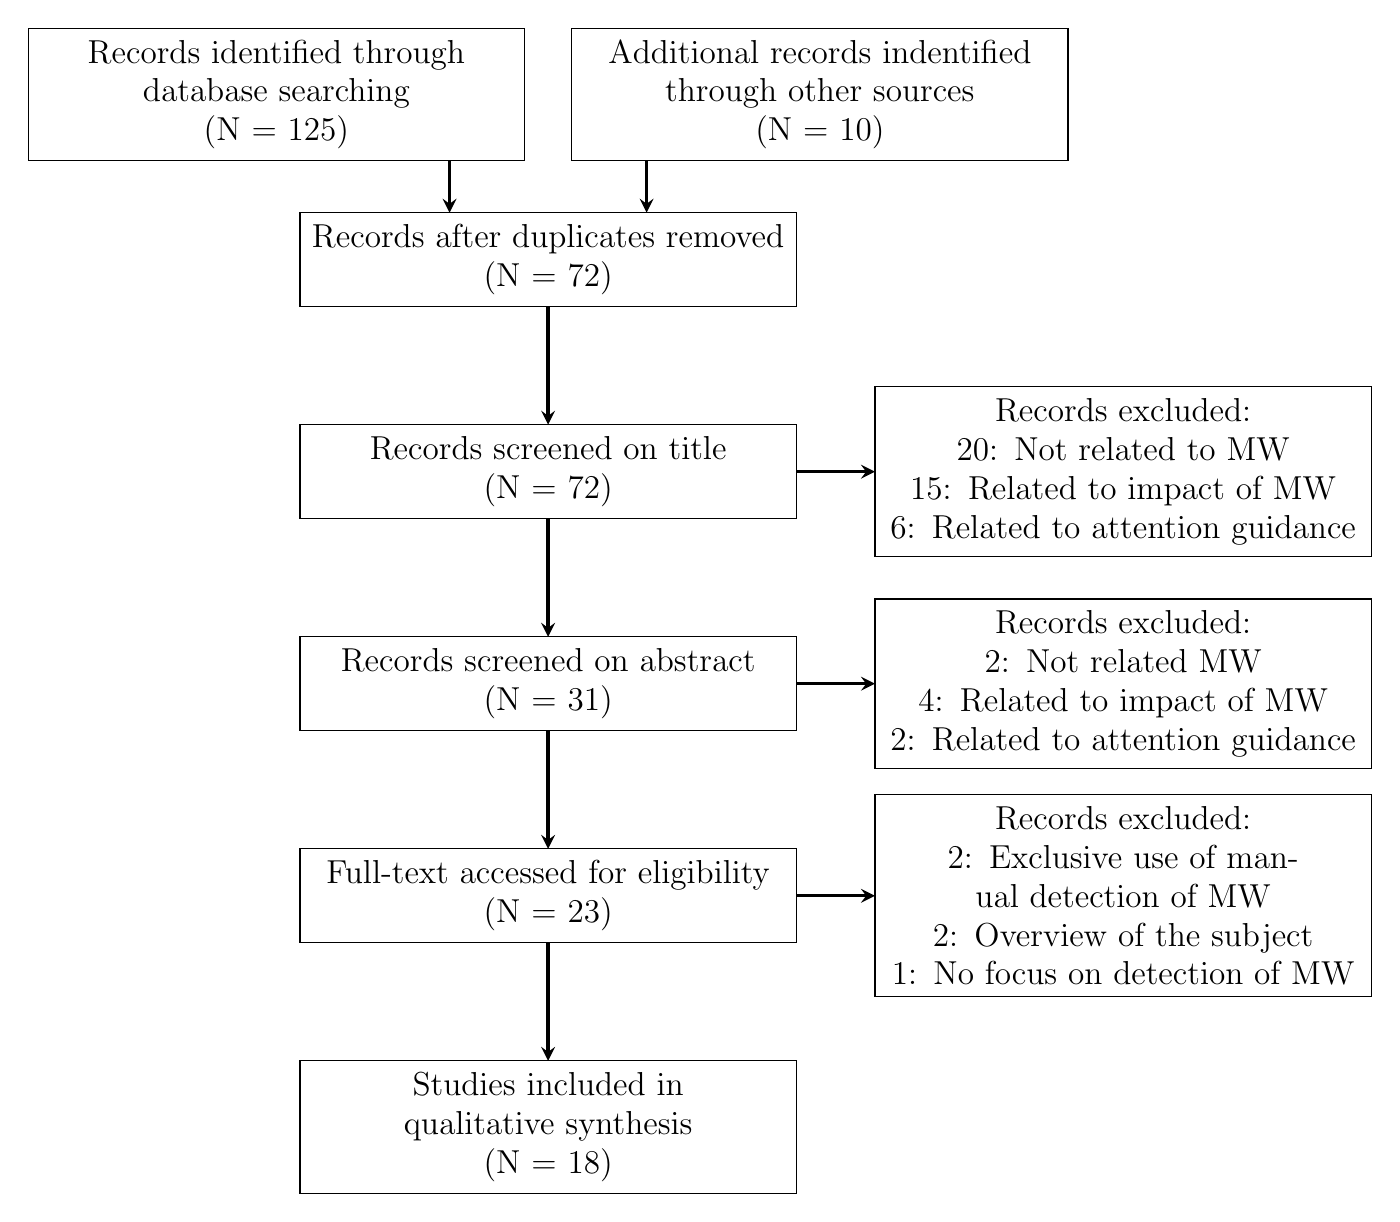
\begin{tikzpicture}[
    node distance=15mm and 10mm,
    start chain=going below,
 mynode/.style = {
        draw, rectangle, align=center, text width=60mm,
        font=\large, inner sep=1ex, outer sep=0pt,
        on chain},
mylabel/.style = {
        draw, rectangle, align=center, rounded corners, 
        font=\small\bfseries, inner sep=2ex, outer sep=0pt,
        fill=cyan!30, minimum height=35mm,
        on chain},
every join/.style = arrow,
     arrow/.style = {very thick,-stealth}
                    ] 
\coordinate (tc);
% the title
%\node[above=of tc,font=\bfseries] {PRISMA 2009 Flow Diagram};
% the nodes at the top
\node (n1a) [mynode, left=of tc, xshift=7mm]    {Records identified through
                                        database searching\\
                                        (N = 125)};
\node (n1b) [mynode,right=of tc, xshift=-7mm]    {Additional records indentified\\
                                        through other sources\\
                                        (N = 10)};
    % the chain in the center
\node (n2)  [mynode, below=of tc]   {Records after duplicates removed\\
                                        (N = 72)};
\node (n3)  [mynode,join]   {Records screened on title\\
                                (N = 72)};
\node (n4)  [mynode,join]   {Records screened on abstract\\
                                (N = 31)};
\node (n5)  [mynode,join]   {Full-text accessed for eligibility\\
                                (N = 23)};
\node (n6)  [mynode,join]   {Studies included in qualitative synthesis\\
                                (N = 18)};
% \node (n7)  [mynode,join]   {\# of studies included in quantitative sysntesis\\
%                                (meta-analysis)};
% the branches to the right
\node (n3r) [mynode,right=of n3]    {Records excluded:\\
                                        20: Not related to MW\\
                                        15: Related to impact of MW\\
                                        6: Related to attention guidance
                                        };
\node (n4r) [mynode,right=of n4]    {Records excluded:\\
                                    2: Not related MW\\
                                    4: Related to impact of MW\\
                                    2: Related to attention guidance
                                    
                                        };
\node (n5r) [mynode,right=of n5]    {Records excluded:\\
                                        2: Exclusive use of manual detection of MW\\
                                        2: Overview of the subject\\
                                        1: No focus on detection of MW};
% lines not included in join                                        
\draw[arrow] ([xshift=+22mm] n1a.south) coordinate (a)
                                       -- (a |- n2.north);
\draw[arrow] ([xshift=-22mm] n1b.south) coordinate (b)
                                       -- (b |- n2.north);
\draw[arrow] (n3) -- (n3r);
\draw[arrow] (n4) -- (n4r);
\draw[arrow] (n5) -- (n5r);
% the labels on the left
%    \begin{scope}[node distance=5mm]
%\node[mylabel,below left=-3mm and 5mm of n1a.north west]
%                {\rotatebox{90}{Identification}};
%\node[mylabel, minimum height=40mm]  {\rotatebox{90}{Screening}};
%\node[mylabel]  {\rotatebox{90}{Eligibility}};
%\node[mylabel]  {\rotatebox{90}{Included}};
%    \end{scope}
\end{tikzpicture}}
\caption{Flow Diagram outlining the screening process}
\label{fig:prisma}
\end{figure}

Second, all duplicates obtained from the different libraries were removed, leaving 72 articles.
Third, from here on after, the articles were divided into two stacks, each containing 36 articles. 
The stacks were peer reviewed on their title. This resulted in three exclusion criteria:
\begin{enumerate}
    \item \textbf{Not related to Mind Wandering}, e.g. \cite{ISI:000432512400017}, focussus on different formats to present lecture material and is therefore excluded.
    \item \textbf{Related to the impact of Mind Wandering}, e.g. \cite{Albert2018LinkingDrivers}, links mind wandering while driving to dangerous behaviour behind the wheel and is thus excluded.
    \item \textbf{Related to attention guidance}, e.g. \cite{Xiao2018ClassroomMechanism}, explores gamification to restore students' attention level in classroom teaching and is thus excluded.
  \end{enumerate}
In case of uncertainty, articles were included to be screened on abstract.
8 articles were excluded while screening on abstract, leaving 23 articles remaining. 
The excluded articles fit the earlier defined exclusion criteria but looked interesting based on the title.

Finally, every remaining article was peer reviewed on their full-text. This included reading the methodology, results, conclusion and inspecting their figures and tables.
Two papers were excluded because they give an overview of the subject, rather than explaining (new) methods of detecting mind wandering. 
Another two articles were excluded since they didn't automatically detect mind wandering, bur rather uses manual (self-)reporting exclusivly.
At last, one article was excluded because it describes a system that uses third party detection mechanisms of mind wandering. The focus of this article lays on implementing this system in a learning environment, rather than on combining/improving detection methods for mind wandering.
The final result is a total of 18 articles to be included in the review.


\subsection{Tasks Evaluated}

\subsection{Features Used}

\subsection{Measuring Mind Wandering}

\subsection{Equipment Used}

\section{Results}

\section{Future Challenges}


\section{Conclusion}

%\end{multicols}
\printbibliography

\end{document}